\documentclass{article}
\usepackage[utf8]{inputenc}
\usepackage{graphicx}
\usepackage{hyperref}
\usepackage{dirtree}
\usepackage[T1]{fontenc}
\usepackage{lmodern}

\begin{document}

\title{Weblab user guide}
\author{Santiago Carot-Nemesio, Raúl Román-López, Jorge Campos Serrano}
\date{\today\\v1.0}

\maketitle

\tableofcontents

\newpage

\begin{abstract}
This document covers the whole installation process of Weblab platform. Weblab is a web based virtualization environment that allow users to create network scenarios enabling them to boot and to configure virtual machines in a decentralized and distributed environment. This document will show you how to get the source code, how to configure it and deploy any module comprising the whole platform so that you can install it in your own environment.
\end{abstract}

\section{Overview}
This section provides a whole view of the Weblab platform. We will describe its architecture and all module which it is composed of.

Weblab is a distributed system that allows users to create and simulate network scenarios. It is designed enabling social interaction such as we tend to see it in social networks, where a single user can create a network scenario and send invitations to other users to join him to solve any exercise. In this way, each scenario can be managed by either a single user or a group of them who can connect to pcs, routers or switches to configure them. Users can boot or shut down virtual machines, which can play the role of a single pc, router or switch, and connect to them using a VT-100 shell console to configure them. All this can be done just using a web browser, no additional software need to be installed on the client computer. Figure \ref{img:weblab_architecture} show all components of the platform and interactions among them.

\begin{figure}[h!]
  \centering
    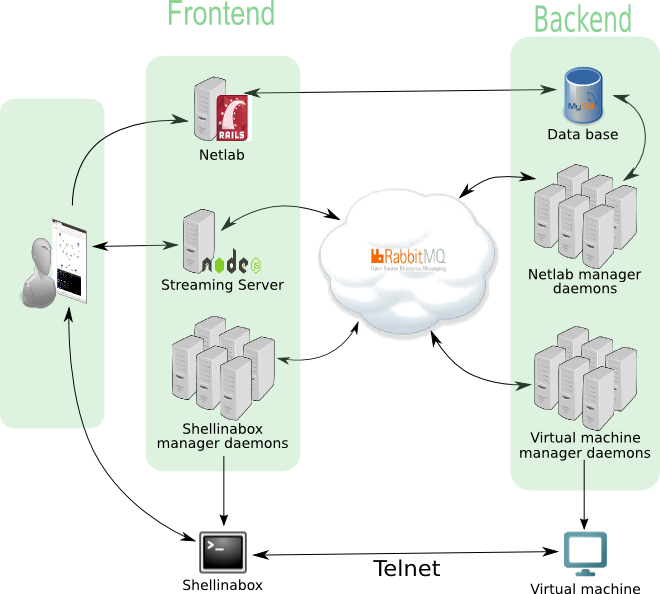
\includegraphics[scale=0.6]{./img/weblab.png}
  \caption{Weblab architecture.}
  \label{img:weblab_architecture}
\end{figure}

In order to accomplish this functionality, Weblab is composed of several modules that can be replicated as much as you want so as to improve reliability. Each module fulfils an specific task that we are going to describe next.

\begin{description}
\item[Netlab] \hfill \\
This is the main component of the front-end. It is a \href{http://rubyonrails.org/}{Rails} web based application which is in charged of managing user accounts, displaying data to users, storing and retrieving user's files in the cloud and so on. It has been developed following a pluggable architecture to ease the development of new features. Plug-ins are developped as Rails \href{http://guides.rubyonrails.org/engines.html}{engines} and they can be integrated in the application as Ruby gems. Netlab provides built-in plug-ins to authenticate user using their Google account and to store files using Google \href{http://www.google.com/drive/about.html?usp=ad_search&gclid=CKW11vPN2bcCFQTHtAodwS4AYw}{drive}, althoug other ones can be also impemented. You will learn how to do it later in section \ref{sec:Development}. It also manages social components which allow users to create groups and network scenarios, send invitations to other users, join to workspaces to simulate and configure networks scenarios, etc.

\item[Streaming server] \hfill \\
This is an \href{http://expressjs.com/}{Express} based server developed in \href{http://nodejs.org/}{Node.js}. Users of the platform connect to this server to get events that happens in the whole system in real time. You will learn how to develop you own source of data later. Up until now, streaming server is used for notifying events involving the state of workspaces. Such kind of events includes unexpected or expected virtual machines crashes, changes in the IP address of any network interface belonging to a certain virtual machine, alerts of connected or disconnected shells, etc. Thanks to this information, Netlab can display asynchronously the updated state of certain workspace on the user's display just as events happen without requiring either pull operations or refreshing the entire web page on the client side. Most of these events arrive in the form of messages that are delivered through \href{http://www.rabbitmq.com/}{RabbitMQ}.

\item[Shellinabox manager daemon] \hfill \\
This is the last component of the front-end. It is a daemon which manages \href{http://code.google.com/p/shellinabox/}{Shellinabox} processes as they are required by the user of the application. Shellinabox implements the javascript VT-100 console so that the web browser can connect to a virtual machine. The connection between the console and the virtual machine is done over Telnet protocol. All paramaters of this connection are internally negotiated between netlab manager daemon and this daemon using RabbitMQ.

\item[Netlab manager daemon] \hfill \\
This is the main component of the back-end. It is responsible of synchronizing the rest of modules connected to message broker, keeping the data base updated with the events that occurs in the system so that the Rails application can present updated data to users. Netlab and this daemon are the only ones that have direct access to the data base. Rest of modules need to synchronize their state retrieving the required information from netlab manager daemon.

\item[Virtual machine manager daemon] \hfill \\
This is the last element of the back-end, It manages workspaces allowing users to start or stop virtual machines when they require it and it is also in charge of sending events that happens on the virtual machines so that Netlab manager daemon can keep the data base updated. This daemon is agnostic from the virtualization technology, it provides a driver based architecture that makes it easy to extend the daemon to provide support for any virtualization technology. Currently it provides a built-in plug-in that manages \href{http://wiki.netkit.org}{Netkit}. Later in section \ref{sec:Development} you will learn how to develop your own driver.
\end{description}

\section{Getting the source code}
\label{sec:Source}
The whole system have been developed using Git. Git is a free and open source distributed version control system designed to handle everything from small to very large projects with speed and efficiency.

Firstly, we need to install this package before we can start downloading the source code. This installation instructions are suited for Linux Ubuntu 12.04 but they might be applied to other Linux distributions although commands and package management tools may differ among Linux distributions.

Type next command as root in order to install the git package. Skip this step if Git is already installed in your system.

\begin{verbatim}
# sudo apt-get install git
\end{verbatim}

Next, we will synchronize all repositories needed to deploy the platform. Source code will be downloaded in /usr/src/weblab but first we are going to create a new group called \textit{weblab} in our system and we will grant read/write permission to it.

\begin{verbatim}
$ sudo addgroup weblab
$ sudo adduser [your_user] weblab
$ sudo mkdir /usr/src/weblab
$ sudo cd /usr/src/weblab
$ sudo chgrp weblab weblab
$ sudo chmod 775 weblab
$ sudo chmod g+s weblab
\end{verbatim}

Replace [your\_user] for the user or users who will be allowed to manipulate the content of this directory. We have set the sticky bit here to grant that all users belonging to \textit{weblab} group can access to read and write files in it.

Go to the /usr/src/weblab directory as a user belonging to \textit{weblab} group and clone all git repositories that you want to install in your machine. Next table shows the repositories and their descriptions:

\begin{center}
\begin{tabular}{|l|r|}
	\hline
$URL$ & $Module$  \\
	\hline
https://github.com/netlab-libresoft/netlab.git   &  Rails front-end application \\
https://github.com/netlab-libresoft/cloudstrg.git   & Generic storage driver for netlab \\
https://github.com/netlab-libresoft/gdrivestrg.git   & Google drive storage plugin  \\
https://github.com/netlab-libresoft/dropboxstrg.git   & Dropbox storage plugin  \\
https://github.com/netlab-libresoft/vmmanager.git   & Virtual machine manager daemon \\
https://github.com/netlab-libresoft/strserver.git   & Streaming server \\
https://github.com/netlab-libresoft/netlabmanager & Netlab manager daemon \\
https://github.com/netlab-libresoft/shellmanager.git & Shellinabox manager daemon \\
	\hline
\end{tabular}
\end{center}

In order to download the source code of any of these modules, just type the command \textit{git clone} followed with the URL where the repository is. Next example shows you how to get the netlab module in the directory /usr/src/weblab.

\begin{verbatim}
$ cd /usr/src/weblab
$ git clone https://github.com/netlab-libresoft/netlab.git
\end{verbatim}

Repeat above operations for each module where you want to get the source code from.

\section{Package dependencies}
This section shows dependencies among Weblab modules and packages that must be installed in your system for them to work.

\subsection{Netlab Web Application}
\label{sub:Netlab} 
Next table shows the list of packages required by this module.

\begin{center}
\begin{tabular}{|l|r|}
	\hline
$Package$ & $Version$  \\
	\hline
RabbitMQ & \textgreater=v3.1.1 \\
Ruby & v1.9.3 \\
Rails & v3.2 \\
https://github.com/netlab-libresoft/cloudstrg.git & development \\
https://github.com/netlab-libresoft/gdrivestrg.git & development  \\
	\hline
\end{tabular}
\end{center}

\subsection{Netlab Manager Daemon}
\label{sub:NetlabManager}
Next table shows the list of packages required by this module.

\begin{center}
\begin{tabular}{|l|r|}
	\hline
$Package$ & $Version$  \\
	\hline
RabbitMQ & \textgreater=v3.1.1 \\
Ruby & v1.9.3 \\
	\hline
\end{tabular}
\end{center}

\subsection{Shellinabox Manager Daemon}
\label{sub:ShellManager}
Next table shows the list of packages required by this module.

\begin{center}
\begin{tabular}{|l|r|}
	\hline
$Package$ & $Version$  \\
	\hline
RabbitMQ & \textgreater=v3.1.1 \\
Ruby & v1.9.3 \\
Shellinabox & \textgreater=v2.10-1 \\
	\hline
\end{tabular}
\end{center}

\subsection{Virtual Machine Manager Daemon}
\label{sub:VMManager}
Next table shows the list of packages required by this module.

\begin{center}
\begin{tabular}{|l|r|}
	\hline
$Package$ & $Version$  \\
	\hline
RabbitMQ & \textgreater=v3.1.1 \\
Node.js & \textgreater=v0.10.8 \\
	\hline
\end{tabular}
\end{center}

Even though virtual machine daemon is agnostic from the virtualization technology, it comes with a built-in plugin that manages Netkit, if you are going to use this plug-in as virtualization technology you will need to fulfil next dependencies too.

\begin{center}
\begin{tabular}{|l|r|}
	\hline
$Package$ & $Version$  \\
	\hline
Netkit core & v2.8 \\
Netkit filesystem & v5.2 \\
Netkit kernel & v2.8 \\
Telnet server & any \\
	\hline
\end{tabular}
\end{center}

\subsection{Streaming server}
\label{sub:StreamingSRV}
Next table shows the list of packages required by this module.

\begin{center}
\begin{tabular}{|l|r|}
	\hline
$Package$ & $Version$  \\
	\hline
RabbitMQ & \textgreater=v3.1.1 \\
Node.js & \textgreater=v0.10.8 \\
	\hline
\end{tabular}
\end{center}

\section{Installation}

This section will show you how to install each module that comprises the Weblab platform, the packages and libraries which they depend on and how to configure them so that you can distribute processes and work in all machines in your environment.

Even though Weblab modules can be installed in a single machine, we strongly recommend you distributing and replicating as many modules as possible so as to improve reliance and load balance in the whole system.

\subsection{RabbitMQ}
\label{sub:RabbitMQInstall}
RabbitMQ is open source message broker software that implements the Advanced Message Queuing Protocol (AMQP) standard.

All Weblab modules use RabbitMQ in order to communicate to one another, send messages, requests and events, so we need to install it before any other component of Weblab environment. To proceed with RabbitMQ installation follow next instruction.

Add the following line to your /etc/apt/sources.list

\begin{verbatim}
deb http://www.rabbitmq.com/debian/ testing main
\end{verbatim}

To avoid warnings about unsigned packages, add the public key to your trusted key list using \textit{apt-key}

\begin{verbatim}
$ wget http://www.rabbitmq.com/rabbitmq-signing-key-public.asc
$ sudo apt-key add rabbitmq-signing-key-public.asc
\end{verbatim}

Update your repositories
\begin{verbatim}
$ sudo apt-get update
\end{verbatim}

Install RabbitMQ package
\begin{verbatim}
$ sudo apt-get install rabbitmq-server
\end{verbatim}

Next we need to configure RabbitMQ to be used for the application. To do that, we need to create a special user and grant permission to him/her.

Let's create the user called \textit{<your-user>} with password \textit{<your-password>}

\begin{verbatim}
$ sudo rabbitmqctl add_user <your-user> <your-password>
\end{verbatim}

Now, we are going to create a virtual host  called \textit{/weblab} for this user so that he can manage resources of any type in there.

\begin{verbatim}
$ sudo rabbitmqctl add_vhost /weblab
\end{verbatim}

Add permission for the user <your-user> in the recently created virtual host.

\begin{verbatim}
sudo rabbitmqctl set_permissions -p /weblab <your-user> ".*" ".*" ".*"
\end{verbatim}

Above command instructs the RabbitMQ broker to grant the user named \textit{<your-user>} access to the virtual host called \textit{/weblab}, with configure, write and read permissions on all resources.

\subsection{Node.js}

Node.js is a platform built on Chrome's JavaScript runtime for easily building fast, scalable network applications. Node.js uses an event-driven, non-blocking I/O model that makes it lightweight and efficient, perfect for data-intensive real-time applications that run across distributed devices.

Both, the streaming server and the virtual machine manager daemon use Node.js, so if you are intending to install one of above mentioned modules in your machine, you will first need to install Node.js before proceeding.

Follow next instructions to install the last stable Node.js package in Ubuntu 12.04. Weblab modules require at least v0.10 to work. The version used when this document was written was v0.10.9.

\begin{verbatim}
$ sudo apt-get update
$ sudo apt-get install python-software-properties python g++ make
$ sudo add-apt-repository ppa:chris-lea/node.js
$ sudo apt-get update
$ sudo apt-get install nodejs
\end{verbatim}

\subsection{Ruby}
Ruby is a dynamic, open source programming language with a focus on simplicity and productivity. It has an elegant syntax that is natural to read and easy to write.

The front end web application, the netlab manager and the shell manager daemons are all written in Ruby. So we will need to install Ruby if we are planning to install one of the above mentioned software components in our machine.

Next instructions will show how to install \textit{rvm} in a multi-user configuration. Make sure you have installed \textit{curl} package before proceeding with the installation.

\begin{verbatim}
$ curl -L https://get.rvm.io | sudo bash -s stable
\end{verbatim}

Add any user you want to manage \textit{rvm} to \textit{rvm} group
\begin{verbatim}
$ sudo adduser [user] rvm
\end{verbatim}

Execute the following command, which provides additional installation instructions tailored to your specific operating system.

\begin{verbatim}
$ rvm requirements
\end{verbatim}

Install the Ruby interpreter itself. All Weblab modules require Ruby 1.9.3.

\begin{verbatim}
$ rvm install 1.9.3
\end{verbatim}

You can also chose to make it the default Ruby interpreter for new terminal sessions with the following command.

\begin{verbatim}
$ rvm --default 1.9.3
\end{verbatim}

\subsection{Rails}
Ruby on Rails is an open source web framework that is optimized for sustainable productivity. It let programmers write beautiful code by favouring convention over configuration.

Rails depends on Ruby, so it is required to install it before continuing this tutorial.

Netlab web application requires Rails v3.2, so if you are planning to deploy Netlab in your machine you will first need to install Rails.

Once Ruby is installed, you have to type next command in a shell.
\begin{verbatim}
$ rvm use 1.9.3
\end{verbatim}

Then, you will be ready to install Rails

\begin{verbatim}
$ gem install rails
\end{verbatim}

Remember that you can set the default Ruby interpreter to 1.9.3 using \textit{rvm --default 1.9.3}

\subsection{Shellinabox}
Shell In A Box implements a web server that can export arbitrary command line tools to a web based terminal emulator. This emulator is accessible to any JavaScript and CSS enabled web browser and does not require any additional browser plugins.

Shellinabox Manager daemon requires it to work, so if you are going to install this module you will first need to install Shellinabox package in your system.

Next section will explain to you how to install Shellinabox package for Ubuntu 12.04. Last stable version of Shellinabox when this document was written was v2.10-1.

Get the Debian package

\begin{verbatim}
$ wget shellinabox.googlecode.com/files/shellinabox_2.10-1_i386.deb
\end{verbatim}

Install it using \textit{dpkg} tool
\begin{verbatim}
$ sudo dpkg -i shellinabox_2.10-1_i386.deb
\end{verbatim}

By default, Shellinabox daemon is configured to start automatically whenever the machine starts, to avoid so, we have to modify default behaviour by editing the configuration file which is in /etc/default/shellinabox. Here we have to set the SHELLINABOX\_DAEMON\_START flag to false.

\begin{verbatim}
...
# Should shellinaboxd start automatically
-SHELLINABOX_DAEMON_START=1
+SHELLINABOX_DAEMON_START=0
...
\end{verbatim}

\subsection{Netkit}
Netkit is an environment for setting up and performing networking experiments at low cost and with little effort. It allows to "create" several virtual network devices (full-fledged routers, switches, computers, etc.) that can be easily interconnected in order to form a network on a single PC. Networking equipments are virtual but feature many of the characteristics of the real ones, including the configuration interface.

Got to /usr/src/weblab and download the Netkit core, filesystem and the kernel files
\begin{verbatim}
$ wget http://wiki.netkit.org/download/netkit/netkit-2.8.tar.bz2
$ wget http://wiki.netkit.org/download/netkit-filesystem/netkit-filesystem-i386-F5.2.tar.bz2
$ wget http://wiki.netkit.org/download/netkit-kernel/netkit-kernel-i386-K2.8.tar.bz2
\end{verbatim}

Unpack them by using next commands
\begin{verbatim}
$ tar -xjSf netkit-x.y.tar.bz2
$ tar -xjSf netkit-filesystem-Fx.y.tar.bz2
$ tar -xjSf netkit-kernel-Kx.y.tar.bz2
\end{verbatim}

Note that all the three packages must be uncompressed while staying in the same directory. It is strongly advised to use the -S option to save space on your disk, because this option handles sparse files (i.e., files with lots of empty blocks) efficiently

Next, we have to configure netkit, in this example, nextkit will be able to be used for all users in the system. To do that, we have to edit the file /etc/bash.bashrc and add next lines at the end of it:

\begin{verbatim}
....
export NETKIT_HOME=/usr/src/weblab/netkit
export MANPATH=:$NETKIT_HOME/man
export PATH=$NETKIT_HOME/bin:$PATH
\end{verbatim}

Now it is time to configure netkit. Before doing it, you must make sure NETKIT\_HOME is already configured in you environment variable type next command in a shell

\begin{verbatim}
$ echo $NETKIT_HOME
/usr/src/weblab/netkit
\end{verbatim}

Above command should show you the PATH where Netkit is installed. If no output is shown, just sign out and sign in again into your shell or type next command \textit{source /etc/bash.bashrc}. The initialization script \textit{bash.bashrc} should set the new environment variables.

Go to the nekit direcotry and execute the configuration script

\begin{verbatim}
$ cd /usr/src/weblab/netkit
$ ./check_configuration.sh
\end{verbatim}

Check out the output in case any dependency should be fulfilled.

Finally, we will need a Telnet server installed in our machine so that Netkit driver can connect to virtual machines. You can install it in Ubuntu using aptitude.

\begin{verbatim}
sudo apt-get install telnetd
\end{verbatim}

\section{Configuration}
This section will show you how to configure any module that composes the platform. As you already know, Weblab is a distributed platform where a group of processes need to connect to one another in order to interchange relevant information regarding where a resource is and how to connect to it. Each Weblab process that is running in any node of your local network need to identify itself in order to make internal configurations about how to connect with any resource it might create, to accomplish that task, all modules resolve the \textit{hostname} in your machine to announce other modules where they are. That \textit{hostname} must be translatable into a IP address by DNS so that other modules can use resources instantiathed by them, such resources can be Shellinaboxes services, virtual machines or any other which requires an IP to connect to.

So you have to configure your host machine to provide a translatable name for any process requiring the \textit{hostname}. Due to the fact that Shellmanager and Virtual machine manager daemons are the only ones that instantiate resources accessible by an IP address, you will only need to configure your \textit{hostname} in the machines you are going to install them. Edit /etc/hostname and provide the DNS name for your machine. In out exampe it will be kenobi.gsyc.es

Here is our /etc/hostname
\begin{verbatim}
$ cat /etc/hostname 
kenobi.gsyc.es
\end{verbatim}

\subsection{Netlab Web Application}
\label{sub:NetlabCFG}
This section will show you how to install and configure the rails web application. Before proceeding, check out that all dependencies required by this module are installed in your machine. You can check them out in the subsection \ref{sub:Netlab}

Netlab uses MySQL, so we also need to install it
\begin{verbatim}
$ sudo apt-get install libmysqlclient-dev mysql-server
\end{verbatim}

Netlab can operate in several execution modes, the more usual ones are development and production, we will use MySQL for above execution modes. First we need to create the data bases for these environments in the server and grant permission to users to access to them. Next command show you how to do it.

\begin{verbatim}
$ mysql -u root -p
mysql> CREATE DATABASE netlab_development;
mysql> GRANT ALL PRIVILEGES ON netlab_development.*
    -> TO '<your-user>'@'localhost' IDENTIFIED BY '<your-password>';

mysql> CREATE DATABASE netlab_production;
mysql> GRANT ALL PRIVILEGES ON netlab_production.*
    -> TO '<your-user>'@'localhost' IDENTIFIED BY '<your-password>';
mysql> EXIT;
\end{verbatim}

Set the user and password you want.

Next, go to /usr/src/weblab/ directory and get the Netlab source code such as it was explained in section \ref{sec:Source}

\begin{verbatim}
$ cd /usr/src/weblab
$ git clone https://github.com/netlab-libresoft/netlab.git
\end{verbatim}

Then, go to Netlab directory and install all gems that this module requires

\begin{verbatim}
$ cd /usr/src/weblab/netlab
$ bundle install
\end{verbatim}

Now it is time to configure the web application. Firstly we have to configure the MySQL parameters so that the netlab application can connect with the MySQL server. In order to do so, we need to modify the content of the file config/database.yml to look like this one

\begin{verbatim}
...
production:
  adapter: mysql2
  encoding: utf8
  reconnect: false
  database: netlab_development
  pool: 5
  username: <your-user>
  password: <your-password>
  timeout: 5000

production:
  adapter: mysql2
  encoding: utf8
  reconnect: false
  database: netlab_production
  pool: 5
  username: <your-user>
  password: <your-password>
  timeout: 5000
...
\end{verbatim}

You have to change the user and password for the ones you set during the MySQL data base configuration step.

Next step consists in migrating the relational schema used by Netlab in MySQL server, to do it, type next command and pulse enter

\begin{verbatim}
$ rake db:migrate
\end{verbatim}

If above command fails telling you to try again using rake, use next command

\begin{verbatim}
$ bundle exec rake db:migrate
\end{verbatim}

By default, development environment will be used. In order to execute migrations for another environment you must provide the RAILS\_ENV variable with environment you want to migrate. Next command will migrate the relational schema for production environment
\begin{verbatim}
$ rake db:migrate RAILS_ENV="production"
\end{verbatim}

Once again, if above command fails, try next one:

\begin{verbatim}
$ bundle exec rake db:migrate RAILS_ENV="production"
\end{verbatim}

If you are deploying in production you will first need to precompile assets as it is explained \href{http://guides.rubyonrails.org/asset_pipeline.html#in-production}{here}. To do that, follow next instructions, if not, you can skip next steps

\begin{verbatim}
$ bundle exec rake assets:precompile
\end{verbatim}

Next, you must enable the flag serve\_static\_assets in the file config/environments/production.rb

\begin{verbatim}
...
config.serve_static_assets = true
...
\end{verbatim}

Sometimes, when you deploy in production, you can experiment problem serving static files, when it happens it is a good idea to reset assets. You can do it with the \textit{clean} option as it is shown next

\begin{verbatim}
$ bundle exec rake assets:clean
$ bundle exec rake assets:precompile
\end{verbatim}

We also need to configure AMQP parameters so that the web application can connect with AMQP server. Modify both, development (config/environments/development.rb) and production (config/environments/production.rb) environments to set proper parameters for your AMQP server. 

Edit AMQP configuration files to set the parameters you set when you installed RabbitMQ, see subsection \ref{sub:RabbitMQInstall} for more details.

Next is our configuration file.

\begin{verbatim}
...
# AMQP configuration object
  config.amqp_settings = {
    :user => "<your-user>",
    :pass => "<your-password>",
    :host => "kenobi.gsyc.es",
    :vhost => "/weblab",
    :heartbeat => 1
  }
...
\end{verbatim}

Next we have to provide an admin account so that Weblab modules can use Netlab REST API. Execute next script and provide all credentials required for your admin account.

You have to change <your-user> and <your-password> for the ones you set
during the RabbitMQ configuration step.

\begin{verbatim}
$ rails generate admin
\end{verbatim}

If you are deploying in production, use next command
\begin{verbatim}
$ RAILS_ENV="production" rails generate admin
\end{verbatim}

Netlab Web Application needs to know the directory where store configuration files, and special files to manage workspaces and virtual machines in your hard drive to download files from each workspace, so you must tell it which directory it should use for that purpose. In our example we are going to use /var/weblab/workspaces.

Edit the file config/initializers/captures\_path.rb and modify it to look like the next one.

\begin{verbatim}
Netlab::Application.config.captures_path = "/var/weblab/workspaces"
\end{verbatim}

That is it. In order to run the Rails application type in a terminal the next command
\begin{verbatim}
$ rails server
\end{verbatim}

The you will be able to connect your web browser to the Netlab web application in the port 3000. Use -e parameter to specify the environment, by default, development is set if nothing else is specified in the command line. To start the server in production simply type next command.


\begin{verbatim}
$ rails server -e production
\end{verbatim}

Type \textit{rails server -h} to get a full list of available options.

Due to some problems regarding redirected URLS with Google drive plugin when Netlab is deployed behind a reverse proxy, we need to configure the file config/initializers/host\_init.rb. Here we must indicate the host, port and url when you are deploying Netlab using a reverse proxy. See section \ref{sec:NGINX} for more details.

We will deploy Netlab with Nginx using the host \textit{kenobi.gsyc.es}, due to the fact we are going to deploy using the port 80 in Nginx, we don't need to tell the port here. We will use HTTP as protocol. Next is the configuration file:

\begin{verbatim}
# This config parameter is used for third-party redirections, 
# where there is a Nginx server scheduling requests

Netlab::Application.config.app_protocol = "http"
Netlab::Application.config.app_host_and_port = "kenobi.gsyc.es"
\end{verbatim}

\subsection{Netlab Manager Daemon}
In this section we are going to install and configure the Netlab manager daemon. Before proceeding, check out that all dependencies required by this module are installed in your machine. You can check them out in the subsection \ref{sub:NetlabManager}

This daemon is responsible of managing the whole state of the system and coordinating all modules connected to the message system. The more netlab manager processes you install, the more reliable the system will be.

First of all, go to /usr/src/weblab directory and get the Netlab manager source code such as it was explained in section \ref{sec:Source}

\begin{verbatim}
$ cd /usr/src/weblab
$ git clone https://github.com/netlab-libresoft/netlabmanager.git
\end{verbatim}

This daemon is implemented over the event machine \href{http://rubyeventmachine.com/}{gem} for ruby, so we will need to install all dependencies before continuing. To do it, go to netlabmanager directory and use \textit{bundle} command to install all gems required by this module.

\begin{verbatim}
$ cd /usr/src/weblab/netlabmanager
$ bundle install
\end{verbatim}

Once again, you will need to configure AMQP settings before starting this daemon. To do it you will have to edit the file config/amqp.yml to set your own settings.

Edit config/mysql.yml to set the user and password for your MySQL environments such as you did in section \ref{sub:NetlabCFG}.

In order to run the daemon, type the following command. Set the proper environment with -e flag. If no flag is provided development environment will be used. Provide -h flag to get a full list of available options.

\begin{verbatim}
$ ./bin/netlabmanager -e production
\end{verbatim}

Check out the section \ref{sub:NetlabManagerBoot} to start this process at boot time.

\subsection{Shellinabox Manager Daemon}
This section will show you how to install and configure the Shellinabox manager daemon. Before proceeding, check out that all dependencies required by this modules are installed in your machine. You can check them out in the subsection \ref{sub:ShellManager}

This daemon is responsible of executing Shellinabox processes in order to connect to a virtual machines when users need it. The more Shellinabox daemons you install, the more scalable the system will be.

Go to /usr/src/weblab directory and get the Netlab manager source code such as it was explained in section \ref{sec:Source}

\begin{verbatim}
$ cd /usr/src/weblab
$ git clone https://github.com/netlab-libresoft/shellmanager.git
\end{verbatim}

Shellinabox manager daemon is also implemented over the event machine \href{http://rubyeventmachine.com/}{gem} for ruby, so we will need to install all dependencies before continuing. To do it, go to Shellmanager directory and use \textit{bundle} command to install all gems required by this module.

\begin{verbatim}
$cd /usr/src/weblab/shellmanager
$ bundle install
\end{verbatim}

Next we have to configure Shellinabox daemon, first of all, we have to set the name of the user who will be used to launch Shellinabox processes on behalf of. Edit the file config/shellmanager.yml and provide the user on the system we want to use. In our example, the Netlab user will be used. No to mention that this user must exist in your machine.

\begin{verbatim}
...
# Shellmanager configuration file

# The configuration specifies the following keys:
# * user     - Shellinabox user name
# * group    - Shellinabox group name
# * path     - Shellinabox configuration directory

defaults: &defaults
  user: <your-user>
  group: <your-group>
  path: /etc/shellinabox
...
\end{verbatim}

Finally, we will also need to configure AMQP parameters so that the daemon can connect with RabbitMQ server. Edit the file config/amqp.yml to provide your own configuration parameters such as you did in previous sections.

Type the following command so as to run the daemon. Remember to set the proper environment with -e flag. If no flag is provided, development environment will be used. Provide -h flag to get a full list of available options.

\begin{verbatim}
$./bin/shellmanager -e production
\end{verbatim}

Check out the section \ref{sub:ShellManagerBoot} to start this process at boot time.

\subsection{Virtual Machine Manager Daemon}
In this section we are going to install and configure the virtual machine manager daemon. Before proceeding, check out that all dependencies required by this module are already installed in your machine. You can check them out in the subsection \ref{sub:VMManager}

This daemon is in charge of starting, stopping and managing virtual machines which belong to any workspace. It has been designed to be agnostic from the virtualization technology. It provides a generic interface called \textit{driver} that let the daemon manage any virtual machine with independence of the underlying virtualization tecnology. Adding a new technology is as easy as to extend the \textit{driver} interface. By the default, Netkit is used but any other could be implemented too.

Go to /usr/src/weblab/ directory and get the virtual machine manager source code such as it was explained in section \ref{sec:Source}

\begin{verbatim}
$ cd /usr/src/weblab
$ git clone https://github.com/netlab-libresoft/vmmanager.git
\end{verbatim}

The virtual machine manager daemon needs to store configuration files, and special files to manage workspaces and virtual machines in your hard drive, so you must tell it which directory it should use for that purpose. In our example we are going to use /var/weblab/workspaces.

Edit the file config/workspace.json and modify it to look like the next one. Make sure that the directory you are going to use exists and read/write permissions are allowed.

\begin{verbatim}
{
  "path": "/var/weblab/workspaces"
}
\end{verbatim}

Because this daemon is based on Node.js, all configuration files will be json files.

We have assigned the group \textit{weblab} to this directory and set the sticky bit too. Remember that you can create a new group using the command \textit{addgroup} in Ubuntu. Next are the command sequence we have done so as to create above directory.

\begin{verbatim}
$ sudo mkdir /var/weblab
$ sudo chgrp weblab /var/weblab
$ sudo chmod g+s /var/weblab
$ sudo mkdir /var/weblab/workspaces
\end{verbatim}

This daemon may need to download workspace associated configuration files by making a GET request to Netlab. Remember that Netlab stores files in the cloud, so such files might be stored in Google Drive, Dropbox, etc. depending on the Storage plug-in used.

Fortunatelly, Netlab provides a REST API that let the daemon get the associated data without worrying about where that file is stored. Virtual machine manager daemon simply make GET requests to Netlab so as to download such kind of files, so all we have to do is to tell the daemon where Netlab application is waiting for requests. Furthermore, the daemon will need to authenticate with Netlab before it can start making requests, so we will configure the daemon to use the admin account we created when we configured the Netlab web application in section \ref{sub:NetlabCFG}. To do that, we have to edit config/rest.json.

In our example, the machine is kenobi.gsyc.es and it will be listening to incoming requests in the port number 80.

\begin{verbatim}
{
  "hostname": "kenobi.gsyc.es",
  "port": 80,
  "path": "/workspaces/:wid/conf",
  "method": "GET",
  "download":"/tmp",
  "authenticate" : {
    "url": "/admins/sign_in",
    "email": "<your-email>",
    "passwd": "<your-password>",
    "cookie": "/usr/src/weblab/session"
  }
}
\end{verbatim}

We must specify the download directory, we have used /tmp, files downloaded will be automatically deleted by the daemon once it has used it.

To finish, edit config/amqp.json to set proper AMQP configuration. Remember that all modules must use the same credentials in order to connect to RabbitMQ to communicate to one another. Here is the one we have used

\begin{verbatim}
{
  "host": "kenobi.gsyc.es",
  "login": "<your-user>",
  "password": "<your-password>",
  "vhost": "/weblab"
}
\end{verbatim}

Remember that host is the machine where RabbitMQ is running.

To run this process execute:

\begin{verbatim}
$ node daemon.js
\end{verbatim}

By default, development environment will be used. To set another environment, you must specify the Node.js NODE\_ENV environment variable. Next example show how to launch the daemon in production.

\begin{verbatim}
$ NODE_ENV=production node daemon.js
\end{verbatim}

Check out the section \ref{sub:VMManagerBoot} to start this process at boot time.

\subsection{Streaming server}
This section will show you how to install and configure the Node.js streaming server. Before proceeding, check out that all dependencies required by this module are already installed in your machine. You can check them out in the subsection \ref{sub:StreamingSRV}

The streaming server has been implemented over Node.js using \href{http://expressjs.com/}{Express} framework. It is used as source of events happening in the platform such as changes of any IP address on any virtual machine, expected or unexpected virtual machines crashes, etc. It uses the new html5 Websockets specification through \href{http://socket.io/}{Socket.io} library to send asynchronous events from the server side to the user's web browser.

To install this module, go to /usr/src/weblab/ directory and get the streaming server source code such as it was explained in section \ref{sec:Source}

\begin{verbatim}
$ cd /usr/src/weblab
$ git clone https://github.com/netlab-libresoft/strserver.git
\end{verbatim}

This server uses Netlab REST API to get user's information using the cookie set by Netlab, in order to this to work, we need, on the one hand, that the cookie is present in headers set by user's web browser, to achieve this, we need that both servers: Netlab and the streaming server are under the same domain, we will do this in section \ref{sec:NGINX}.

On the other hand, we have to configure the streaming server to use the Netlab REST API to get user's information. To do that we have to edit the configuration file config/authorize.json to tell the server where Netlab is waiting for requests.

Here it is our configuration file
\begin{verbatim}
{
  "hostname": "kenobi.gsyc.es",
  "port": 80,
  "path": "/profiles/info.json",
  "key": null,
  "cert": null,
  "ca": null,
  "method": "GET"
}
\end{verbatim}

As you can see, we can set the server certification in the configuration file in case Netlab is working over SSL, but this feature is not yet implemented.

We also have to configure AMQP so that it can send messages to other modules in the platform. Remember that the user should be the same for all modules.

AMQP configuration file is config/amqp.json. Here it is the one used in our example:
\begin{verbatim}
{
  "host": "kenobi.gsyc.es",
  "login": "<your-user>",
  "password": "<your-password>",
  "vhost": "/weblab"
}
\end{verbatim}

To run this process execute:

\begin{verbatim}
$ node server.js
\end{verbatim}

From now, you will be able to connect to the streaming server in the port number 9000. You can check that everything is al-right loading the test page server from /. In our example it will be kenobi.gsyc.es:9000/

To change the port number, edit the file server.js and change the variables port and hostname that are at the beginning.

By default, development environment will be used. To set another environment, you must specify the Node.js NODE\_ENV environment variable. Next example show how to launch the daemon in production.

\begin{verbatim}
$ NODE_ENV=production node server.js
\end{verbatim}

Check out the section \ref{sub:StreamingSRVBoot} to start this process at boot time.

\section{Deploying with Nginx}
\label{sec:NGINX}

Weblab is a distributed web application that comprises several modules, among them, two web servers: Netlab and the Streaming server. The first one is the user front-end which is written in \href{http://rubyonrails.org/}{Rails}. This web application manages user's accounts allowing them to log-in to create and manage virtual machines. The second server, is a Node.js based one that is used for sending events concerning virtual machine state changes, ip changes and so on in real time. So that the system could work properly, it is required for both servers to operate under the same domain. In order to accomplish this task, we will use \href{http://nginx.org/}{Nginx} to redirect requests to one or another server depending on the URL used to make the request. URLS starting either with /socket.io or /streaming will be redirected to the Streaming server whereas the rest of requests which do not match the former criteria will be redirected to Netlab server.

Ruby on Rails is an application stack that provides web developers with a framework to quickly create a variety of web applications, and Nginx is a light, high performance web server software. The two programs can be easily configured to work very well together on a virtual private server when installed through \href{www.phusionpassenger.com}{Phusion Passenger}.

Passenger is an effective and easy way to deploy Rails on Nginx or Apache. In this instance, we are going to run the nginx installation. 

Nginx is a different from other web servers in that it does not support loadable modules. The only way to extend Nginx is to recompile it entirely from source. Since Phusion Passenger consists of some external executables plus an Nginx module, you must recompile Nginx when first installing Phusion Passenger, but also when upgrading Nginx itself or when upgrading the Phusion Passenger version.

Go ahead and install passenger.
\begin{verbatim}
$ gem install passenger
\end{verbatim}

To proceed with installing or upgrading Phusion Passenger, run the Phusion Passenger Nginx installer and follow the on-screen instructions

\begin{verbatim}
$ rvmsudo passenger-install-nginx-module
\end{verbatim}

This installation program will offer you two installation modes, automatic or manual. We have chosen the automatic one. Whatever you choose, make sure Nginx version installed is at least 1.4, because lower ones do not provide support for Websockets which is required by the Streaming server in order to use real time notifications.

The Nginx configuration file we have chosen is /opt/nginx/conf/nginx.conf. The installer will have modified the configuration file by setting the correct options so that Phusion Passenger can work correctly. The following configuration snippet will have been inserted

\begin{verbatim}
  http {
      ...
      passenger_root /usr/local/rvm/gems/ruby-1.9.3-p429/gems/passenger-4.0.5;
      passenger_ruby /usr/local/rvm/wrappers/ruby-1.9.3-p429/ruby;
      ...
  }
\end{verbatim}

After you start Nginx, you will be ready to deploy any number of Ruby on Rails applications on Nginx.

By default, Nginx does not start at boot time, so if you want it to do so, go to the section \ref{sub:NginxBoot} to see how to do it.

Next, we have to configure Nginx to redirect requests to Netlab web application. Create a sites-enabled folder in the \textit{conf} subdirectory which is under your Nginx installation directory.

\begin{verbatim}
$ sudo mkdir /opt/nginx/conf/sites-enabled
\end{verbatim}

Create a new file called netlab.conf in it with the next content. Make sure your path point to your Netlab installation directory.

\begin{verbatim}
server {
    listen 127.0.0.1:3000;
    #server_name localhost;

    passenger_enabled on;
    rails_env production;

    passenger_spawn_method conservative;

    root /usr/src/weblab/netlab/public;
}
\end{verbatim}

Then, we are going to make proper redirections based on the URL requested. Remember that URLs starting either with /socket.io or /streaming will be redirected to the Streaming server and the rest of requests will be redirected to Netlab server.

Copy next configuration file in conf/nginx.conf from your Nginx installation directory

\begin{verbatim}
#user  nobody;
worker_processes  1;

#error_log  logs/error.log;
#error_log  logs/error.log  notice;
#error_log  logs/error.log  info;

#pid        logs/nginx.pid;


events {
    worker_connections  1024;
}


http {
    passenger_root /usr/local/rvm/gems/ruby-1.9.3-p429/gems/passenger-4.0.5;
    passenger_ruby /usr/local/rvm/wrappers/ruby-1.9.3-p429/ruby;

    include       mime.types;
    default_type  application/octet-stream;

    #log_format  main  '$remote_addr - $remote_user [$time_local] "$request" '
    #                  '$status $body_bytes_sent "$http_referer" '
    #                  '"$http_user_agent" "$http_x_forwarded_for"';

    #access_log  logs/access.log  main;

    sendfile        on;
    #tcp_nopush     on;

    #keepalive_timeout  0;
    keepalive_timeout  65;

    #gzip  on;

    server {
        listen       80;
        server_name  localhost;

        #charset koi8-r;

        #access_log  logs/host.access.log  main;

        location / {
            proxy_set_header X-Real-IP $remote_addr;
            proxy_set_header X-Forwarded-For $proxy_add_x_forwarded_for;
            proxy_set_header Host $http_host;
            proxy_set_header X-NginX-Proxy true;
            proxy_pass http://127.0.0.1:3000/;
            proxy_redirect off;
        }

        location /socket.io {
          proxy_pass http://127.0.0.1:9000;
          proxy_redirect off;

          proxy_http_version 1.1;
          proxy_set_header Upgrade $http_upgrade;
          proxy_set_header Connection "upgrade";
        }

        location /streaming/{
          proxy_set_header X-Real-IP $remote_addr;
          proxy_set_header X-Forwarded-For $proxy_add_x_forwarded_for;
          proxy_set_header Host $http_host;
          proxy_set_header X-NginX-Proxy true;
          proxy_pass http://127.0.0.1:9000/;
          proxy_redirect off;

          proxy_http_version 1.1;
          proxy_set_header Upgrade $http_upgrade;
          proxy_set_header Connection "upgrade";
        }
    }

    include sites-enabled/*.conf;
}
\end{verbatim}

That is it, make sure that both, netlab and the streaming server are up before making any request. You can configure them to start automatically at boot time. For more information, check out the sections \ref{sub:StreamingSRVBoot} and \ref{sub:NginxBoot}.

\section{Starting daemons at boot time}
This section will show you how to deploy the platform so as to set up all daemons whenever a machine starts. This is an helpful mechanism to grant that every single process is up after any single machine crashes or reboots. As you will see, we will create an initialization script to manage each daemon that we will place in an specific directory in your operating system in order to boot it whenever the machine boots.


\label{sec:Boot}

\subsection{Streaming server init script}
\label{sub:StreamingSRVBoot}
This section will show you how to configure Express Streaming server to run at boot time. We will use \href{https://github.com/nodejitsu/forever}{Forever} to it. Forever is a useful tool for running a Node.js process with monitoring capabilities; it can be set to restart a failed process, and has a few other helpful features along the same lines which we will use for our init script.

Forever must be installed globally via NPM for the scripts to work

\begin{verbatim}
$ sudo npm install -g forever
\end{verbatim}

Next, create a script file called streamingsrv with the next content.
 
\begin{verbatim}
#!/bin/bash

### BEGIN INIT INFO
# Provides:             streamingsrv
# Required-Start:       $syslog $remote_fs
# Required-Stop:        $syslog $remote_fs
# Should-Start:         $local_fs
# Should-Stop:          $local_fs
# Default-Start:        2 3 4 5
# Default-Stop:         0 1 6
# Short-Description:    starts the streaming server web server
# Description:          starts streaming server using start-stop-daemon
### END INIT INFO
 

NAME="Streaming server"
NODE_BIN_DIR=/usr/bin
NODE_PATH=/usr/lib/node_modules
NODE_ENV=production
APPLICATION_DIRECTORY=/usr/src/weblab/strserver
APPLICATION_START=server.js
PIDFOLDER=/var/run/netlab
LOGFOLDER=/var/log/netlab
PIDFILE=/var/run/netlab/streamingsrv.pid
LOGFILE=/var/log/netlab/streamingsrv.log
USER=<your-user>

 
# Add node to the path for situations in which the environment is passed.
PATH=$NODE_BIN_DIR:$PATH

# Export all environment variables that must be visible for the Node.js
# application process forked by Forever. It will not see any of the other
# variables defined in this script.
export NODE_PATH=$NODE_PATH

# Set node environment
export NODE_ENV=$NODE_ENV

if [ ! -d $PIDFOLDER ] ; then
    sudo mkdir -p $PIDFOLDER
    sudo chown $USER:$USER $PIDFOLDER
fi

if [ ! -d $LOGFOLDER ] ; then
    sudo mkdir -p $LOGFOLDER
    sudo chown $USER:$USER $LOGFOLDER
fi

start() {
    echo "Starting $NAME"
    # We're calling forever directly without using start-stop-daemon for the
    # sake of simplicity when it comes to environment, and because this way
    # the script will work whether it is executed directly or via the service
    # utility.
    #
    # The minUptime and spinSleepTime settings stop Forever from thrashing if
    # the application fails immediately on launch. This is generally necessary to
    # avoid loading development servers to the point of failure every time
    # someone makes an error in application initialization code, or bringing down
    # production servers the same way if a database or other critical service
    # suddenly becomes inaccessible.
    #
    # The pidfile contains the child process pid, not the forever process pid.
    # We're only using it as a marker for whether or not the process is
    # running.
    forever --pidFile $PIDFILE --sourceDir $APPLICATION_DIRECTORY \
        -a -l $LOGFILE --minUptime 5000 --spinSleepTime 2000 \
        start $APPLICATION_START &
    RETVAL=$?
}
 
stop() {
    if [ -f $PIDFILE ]; then
        echo "Shutting down $NAME"
        # Tell Forever to stop the process. Note that doing it this way means
        # that each application that runs as a service must have a different
        # start file name, regardless of which directory it is in.
        forever stop $APPLICATION_START
        # Get rid of the pidfile, since Forever won't do that.
        rm -f $PIDFILE
        RETVAL=$?
    else
        echo "$NAME is not running."
        RETVAL=0
    fi
}
 
restart() {
    echo "Restarting $NAME"
    stop
    start
}
 
status() {
    echo "Status for $NAME:"
    # This is taking the lazy way out on status, as it will return a list of
    # all running Forever processes. You get to figure out what you want to
    # know from that information.
    #
    # On Ubuntu, this isn't even necessary. To find out whether the service is
    # running, use "service my-application status" which bypasses this script
    # entirely provided you used the service utility to start the process.
    forever list
    RETVAL=$?
}
 
case "$1" in
    start)
        start
        ;;
    stop)
        stop
        ;;
    status)
        status
        ;;
    restart)
        restart
        ;;
    *)
        echo "Usage: {start|stop|status|restart}"
        exit 1
        ;;
esac
exit $RETVAL
\end{verbatim}

Make sure that all paths used in it match with your streaming server installation.

Next we have to copy this script to /etc/init.d and give execution permission to it. Follow next steps to configure your system to start the streaming server at boot time.

\begin{verbatim}
$ sudo cp streamingsrv /etc/init.d/streamingsrv
$ sudo chmod a+x /etc/init.d/streamingsrv
$ sudo update-rc.d streamingsrv defaults
\end{verbatim}

Run or check on the script and its process with the following commands:

\begin{verbatim}
sudo -u <your-user> service streamingsrv start
sudo -u <your-user> service streamingsrv status
sudo -u <your-user> service streamingsrv restart
sudo -u <your-user> service streamingsrv stop
\end{verbatim}

\subsection{Nginx init script}
\label{sub:NginxBoot}
In this section, we are going to create an initialization script for Nginx which allows us to start, stop or restart it. Next we will install it so that it can be automatically started whenever the computer starts during the initialization phase.

Copy next script in a file called Nginx. Make sure that all routes used for the PATH and DAEMON variables match with your Nginx installation.

\begin{verbatim}
#! /bin/sh

### BEGIN INIT INFO
# Provides:          nginx
# Required-Start:    $all
# Required-Stop:     $all
# Default-Start:     2 3 4 5
# Default-Stop:      0 1 6
# Short-Description: starts the nginx web server
# Description:       starts nginx using start-stop-daemon
### END INIT INFO

PATH=/opt/nginx/sbin:/sbin:/bin:/usr/sbin:/usr/bin
DAEMON=/opt/nginx/sbin/nginx
NAME=nginx
DESC=nginx

test -x $DAEMON || exit 0

# Include nginx defaults if available
if [ -f /etc/default/nginx ] ; then
        . /etc/default/nginx
fi

set -e

case "$1" in
  start)
        echo -n "Starting $DESC: "
        start-stop-daemon --start --quiet --pidfile /opt/nginx/logs/$NAME.pid \
                --exec $DAEMON -- $DAEMON_OPTS
        echo "$NAME."
        ;;
  stop)
        echo -n "Stopping $DESC: "
        start-stop-daemon --stop --quiet --pidfile /opt/nginx/logs/$NAME.pid \
                --exec $DAEMON
        echo "$NAME."
        ;;
  restart|force-reload)
        echo -n "Restarting $DESC: "
        start-stop-daemon --stop --quiet --pidfile \
                /opt/nginx/logs/$NAME.pid --exec $DAEMON
        sleep 1
        start-stop-daemon --start --quiet --pidfile \
                /opt/nginx/logs/$NAME.pid --exec $DAEMON -- $DAEMON_OPTS
        echo "$NAME."
        ;;
  reload)
          echo -n "Reloading $DESC configuration: "
          start-stop-daemon --stop --signal HUP --quiet \
              --pidfile /opt/nginx/logs/$NAME.pid --exec $DAEMON
          echo "$NAME."
          ;;
      *)
            N=/etc/init.d/$NAME
            echo "Usage: $N {start|stop|restart|reload|force-reload}" >&2
            exit 1
            ;;
    esac

    exit 0
\end{verbatim}

If you are using ubuntu 12.04 you can follow next steps to above init script

\begin{verbatim}
$ wget -O init-deb.sh http://library.linode.com/assets/1139-init-deb.sh
\end{verbatim}

Next we have to copy this script to /etc/init.d and give execution permission to it. Follow next steps to configure your system to start Nginx at boot time.

\begin{verbatim}
$ sudo mv init-deb.sh /etc/init.d/nginx
$ sudo chmod +x /etc/init.d/nginx
$ sudo /usr/sbin/update-rc.d -f nginx defaults
\end{verbatim}

To start nginx type next command.

\begin{verbatim}
$ sudo service nginx start
\end{verbatim}

Now you can connect to your web server and see \textbf{“Welcome to nginx”} screen in your browser if you point it toward http://youripaddress/

To verify that Phusion Passenger is running
\begin{verbatim}
$ passenger-memory-stats
\end{verbatim}

\subsection{Netlab manager init script}
\label{sub:NetlabManagerBoot}
This daemon is in responsible of keeping the whole state of the system updated by watching at the messages interchanged and events that happens in the message system. In this section we will make it start automatically at boot time.

To manage this process in Ubuntu, create a file called netlabmanager with the next content

\begin{verbatim}
#!/bin/bash

### BEGIN INIT INFO
# Provides:             netlabmanager
# Required-Start:       $syslog $remote_fs
# Required-Stop:        $syslog $remote_fs
# Should-Start:         $local_fs
# Should-Stop:          $local_fs
# Default-Start:        2 3 4 5
# Default-Stop:         0 1 6
# Short-Description:    starts netlabmanager daemon
# Description:          starts netlabmanager daemon using start-stop-daemon
### END INIT INFO
 

NAME="netlabmanager"
ENV=production
APPLICATION_DIRECTORY=/usr/src/weblab/netlabmanager
PIDFOLDER=/var/run/netlab
LOGFOLDER=/var/log/netlab
PIDFILE=/var/run/netlab/netlabmanager.pid
LOGFILE=/var/log/netlab/netlabmanager.log
USER=<your-user>


#source /etc/profile
type rvm >/dev/null 2>/dev/null || echo ${PATH} | GREP_OPTIONS="" \
   grep "/usr/local/rvm/bin" > /dev/null || export PATH="${PATH}:/usr/local/rvm/bin"

if [ ! -d $PIDFOLDER ] ; then
    sudo mkdir -p $PIDFOLDER
    sudo chown $USER:$USER $PIDFOLDER
fi

if [ ! -d $LOGFOLDER ] ; then
    sudo mkdir -p $LOGFOLDER
    sudo chown $USER:$USER $LOGFOLDER
fi

start() {
    echo "Starting $NAME"
    cd $APPLICATION_DIRECTORY
    ./bin/$NAME start -e $ENV -p $PIDFILE -l $LOGFILE
    RETVAL=$?
}
 
stop() {
    if [ -f $PIDFILE ]; then
        echo "Shutting down $NAME"
        cd $APPLICATION_DIRECTORY
        echo "Executing"
        ./bin/$NAME stop -p $PIDFILE
        RETVAL=$?
    else
        echo "$NAME is not running."
        RETVAL=0
    fi
}
 
restart() {
    echo "Restarting $NAME"
    stop
    start
}
 
status() {
    echo "Status for $NAME:"
    if [ -f $PIDFILE ]; then
        echo "$NAME is running with pid:"
        cat $PIDFILE
        RETVAL=$?
    else
        echo "$NAME is not running."
        RETVAL=0
    fi
}
 
case "$1" in
    start)
        start
        ;;
    stop)
        stop
        ;;
    status)
        status
        ;;
    restart)
        restart
        ;;
    *)
        echo "Usage: {start|stop|status|restart}"
        exit 1
        ;;
esac
exit $RETVAL
\end{verbatim}

Make sure that all paths used in this script match with your Netlab manager daemon installation.

Next, follow next steps to complete the installation

\begin{verbatim}
$ sudo cp netlabmanager /etc/init.d/netlabmanager
$ sudo chmod a+x /etc/init.d/netlabmanager
$ sudo update-rc.d netlabmanager defaults
\end{verbatim}

From now, you will be able to manage the daemon using next command

\begin{verbatim}
sudo -u <your-user> service netlabmanager start
sudo -u <your-user> service netlabmanager status
sudo -u <your-user> service netlabmanager restart
sudo -u <your-user> service netlabmanager stop
\end{verbatim}

\subsection{Shellmanager init script}
\label{sub:ShellManagerBoot}
This section will show you how to install the Shellmanager daemon to start at booting time. This daemon allows users to start Shellinabox processes to connect to virtual machines from a web browser. This installation process is quite similar to the one explained above for Netlabmanager process.

First, create a file called shellmanager adding the next content to it.

\begin{verbatim}
#!/bin/bash

### BEGIN INIT INFO
# Provides:             shellmanager
# Required-Start:       $syslog $remote_fs
# Required-Stop:        $syslog $remote_fs
# Should-Start:         $local_fs
# Should-Stop:          $local_fs
# Default-Start:        2 3 4 5
# Default-Stop:         0 1 6
# Short-Description:    starts shellmanager daemon
# Description:          starts shellmanager daemon using start-stop-daemon
### END INIT INFO
 

NAME="shellmanager"
ENV=production
APPLICATION_DIRECTORY=/usr/src/weblab/shellmanager
PIDFOLDER=/var/run/netlab
LOGFOLDER=/var/log/netlab
PIDFILE=/var/run/netlab/shellmanager.pid
LOGFILE=/var/log/netlab/shellmanager.log
USER=<your-user>


type rvm >/dev/null 2>/dev/null || echo ${PATH} | GREP_OPTIONS="" \
   grep "/usr/local/rvm/bin" > /dev/null || export PATH="${PATH}:/usr/local/rvm/bin"

if [ ! -d $PIDFOLDER ] ; then
    sudo mkdir -p $PIDFOLDER
    sudo chown $USER:$USER $PIDFOLDER
fi

if [ ! -d $LOGFOLDER ] ; then
    sudo mkdir -p $LOGFOLDER
    sudo chown $USER:$USER $LOGFOLDER
fi

start() {
    echo "Starting $NAME"
    cd $APPLICATION_DIRECTORY
    ./bin/$NAME start -e $ENV -p $PIDFILE -l $LOGFILE
    RETVAL=$?
}
 
stop() {
    if [ -f $PIDFILE ]; then
        echo "Shutting down $NAME"
        cd $APPLICATION_DIRECTORY
        echo "Executing"
        ./bin/$NAME stop -p $PIDFILE
        RETVAL=$?
    else
        echo "$NAME is not running."
        RETVAL=0
    fi
}
 
restart() {
    echo "Restarting $NAME"
    stop
    start
}
 
status() {
    echo "Status for $NAME:"
    if [ -f $PIDFILE ]; then
        echo "$NAME is running with pid:"
        cat $PIDFILE
        RETVAL=$?
    else
        echo "$NAME is not running."
        RETVAL=0
    fi
}
 
case "$1" in
    start)
        start
        ;;
    stop)
        stop
        ;;
    status)
        status
        ;;
    restart)
        restart
        ;;
    *)
        echo "Usage: {start|stop|status|restart}"
        exit 1
        ;;
esac
exit $RETVAL
\end{verbatim}

Once again, make sure that all paths used for this script match with ones regarding your Shellinabox manager daemon installation.

Next, follow next steps to complete the installation

\begin{verbatim}
$ sudo cp shellmanager /etc/init.d/shellmanager
$ sudo chmod a+x /etc/init.d/shellmanager
$ sudo update-rc.d shellmanager defaults
\end{verbatim}

From now, you will be able to manage the daemon using next command

\begin{verbatim}
sudo -u <your-user> service shellmanager start
sudo -u <your-user> service shellmanager status
sudo -u <your-user> service shellmanager restart
sudo -u <your-user> service shellmanager stop
\end{verbatim}

\subsection{virtual machine manager init script}
\label{sub:VMManagerBoot}
This section will show you how to make virtual machine manager process start at booting time. We will use Forever again such as we did in section \ref{sub:StreamingSRVBoot} to execute the Streaming server at boot time. As we explained, Forever is well suited to manage Node.js process, so install it if you have not done it yet.

\begin{verbatim}
$ sudo npm install -g forever
\end{verbatim}

Next, create a script file called vmmanager with the next content.

\begin{verbatim}
#!/bin/bash

### BEGIN INIT INFO
# Provides:             vmmanager
# Required-Start:       $syslog $remote_fs
# Required-Stop:        $syslog $remote_fs
# Should-Start:         $local_fs
# Should-Stop:          $local_fs
# Default-Start:        2 3 4 5
# Default-Stop:         0 1 6
# Short-Description:    starts virtual machine manager daemon
# Description:          starts virtual machine manager daemon
### END INIT INFO
 

NAME="virtual machine manager daemon"
NODE_BIN_DIR=/usr/bin
NODE_PATH=/usr/lib/node_modules
NODE_ENV=production
APPLICATION_DIRECTORY=/usr/src/weblab/vmmanager
APPLICATION_START=daemon.js
PIDFOLDER=/var/run/netlab
LOGFOLDER=/var/log/netlab
PIDFILE=/var/run/netlab/vmmanager.pid
LOGFILE=/var/log/netlab/vmmanager.log
USER=<your-user>

 
# Add node to the path for situations in which the environment is passed.
PATH=$NODE_BIN_DIR:$PATH

export NETKIT_HOME=/usr/src/weblab/netkit
export MANPATH=:$NETKIT_HOME/man
export PATH=$NETKIT_HOME/bin:$PATH

# Export all environment variables that must be visible for the Node.js
# application process forked by Forever. It will not see any of the other
# variables defined in this script.
export NODE_PATH=$NODE_PATH

# Set node environment
export NODE_ENV=$NODE_ENV

if [ ! -d $PIDFOLDER ] ; then
    sudo mkdir -p $PIDFOLDER
    sudo chown $USER:$USER $PIDFOLDER
fi

if [ ! -d $LOGFOLDER ] ; then
    sudo mkdir -p $LOGFOLDER
    sudo chown $USER:$USER $LOGFOLDER
fi
 
start() {
    echo "Starting $NAME"
    # We're calling forever directly without using start-stop-daemon for the
    # sake of simplicity when it comes to environment, and because this way
    # the script will work whether it is executed directly or via the service
    # utility.
    #
    # The minUptime and spinSleepTime settings stop Forever from thrashing if
    # the application fails immediately on launch. This is generally necessary to
    # avoid loading development servers to the point of failure every time
    # someone makes an error in application initialization code, or bringing down
    # production servers the same way if a database or other critical service
    # suddenly becomes inaccessible.
    #
    # The pidfile contains the child process pid, not the forever process pid.
    # We're only using it as a marker for whether or not the process is
    # running.
    forever --pidFile $PIDFILE --sourceDir $APPLICATION_DIRECTORY \
        -a -l $LOGFILE --minUptime 5000 --spinSleepTime 2000 \
        start $APPLICATION_START &
    RETVAL=$?
}
 
stop() {
    if [ -f $PIDFILE ]; then
        echo "Shutting down $NAME"
        # Tell Forever to stop the process. Note that doing it this way means
        # that each application that runs as a service must have a different
        # start file name, regardless of which directory it is in.
        forever stop $APPLICATION_START
        # Get rid of the pidfile, since Forever won't do that.
        rm -f $PIDFILE
        RETVAL=$?
    else
        echo "$NAME is not running."
        RETVAL=0
    fi
}
 
restart() {
    echo "Restarting $NAME"
    stop
    start
}
 
status() {
    echo "Status for $NAME:"
    # This is taking the lazy way out on status, as it will return a list of
    # all running Forever processes. You get to figure out what you want to
    # know from that information.
    #
    # On Ubuntu, this isn't even necessary. To find out whether the service is
    # running, use "service my-application status" which bypasses this script
    # entirely provided you used the service utility to start the process.
    forever list
    RETVAL=$?
}
 
case "$1" in
    start)
        start
        ;;
    stop)
        stop
        ;;
    status)
        status
        ;;
    restart)
        restart
        ;;
    *)
        echo "Usage: {start|stop|status|restart}"
        exit 1
        ;;
esac
exit $RETVAL
\end{verbatim}

Make sure that all paths used for this script match with ones regarding your virtual machine manager daemon installation.

Next, follow next steps to complete the installation

\begin{verbatim}
$ sudo cp vmmanager /etc/init.d/vmmanager
$ sudo chmod a+x /etc/init.d/vmmanager
$ sudo update-rc.d vmmanager defaults
\end{verbatim}

From now, you will be able to manage the daemon using next command

\begin{verbatim}
sudo -u <your-user> service vmmanager start
sudo -u <your-user> service vmmanager status
sudo -u <your-user> service vmmanager restart
sudo -u <your-user> service vmmanager stop
\end{verbatim}

\section{Development}
\label{sec:Development}
This section will introduce to you the main parts and key concepts to start developing new features. As you have seen, the platform comprises several modules, each one has its own internal structure and software interfaces that you must know in order to develop code efficiently. Here you will learn how to extend the system to create new plug-ins that will allow users to save their data in any cloud technology you want, make authentication process using web services, or to provide any new features you could imagine so as to fulfil any new requirement, from proving a new streaming source of data to create a ew driver to manage any new virtualization technology..

All modules in the system except for Netlab are implemented according the \href{http://www.dre.vanderbilt.edu/~schmidt/PDF/reactor-siemens.pdf}{reactor pattern}. This is such a common design pattern for event-driven applications which require high-performance I/O operations, so you must be familiarized with it to avoid blocking the server making long synchronized I/O operations of any kind.
 
\subsection{Storage plugin}
The cloud storage system for Ruby on Rails, henceforth RoR, is made up of a collection of engine-mode plugins that let users store files such as scenes or configuration files from the Netlab context to the cloud system. So far, Google Drive and Dropbox plug-ins are supported, but other ones can also be implemented.

Storage plug-ins follows a common interface that makes the integration process transparent to Netlab developers. The structure of the cloud storage plug-in system is so simple. On the one hand, there is a basic plug-in, called \textit{Cloudstrg}, which includes the main interface definition class that all storage plug-ins must inherit from, plus some methods defined in this class so as to list installed plug-ins in order to instantiate the required one. On the other hand, there is a collection of extended plug-ins which follow the unified interface where each one manages their specific data internally. These plug-ins are developed using the \href{http://guides.rubyonrails.org/engines.html}{engine} plug-in mechanism, that makes them independent from the main application by implementing their own models, migration scrips, tables, views and controllers that can be mounted on the host application.

Check out the section \ref{sec:Source} to get more information regarding how to get the source code. It includes proper documentation concerning the methods that all plug-ins that inherit from \textit{Cloudstrg} must implement.

The file /lib/cloudstrg/cloudstrg.rb in \textit{Cloudstrg} repository, defines the above mentioned interface that plug-ins inheriting from it should implement in order to create, delete, update and share files in the cluod. This plug-in provides three models to users that let them configure the way they will use the cloud storage system:

\begin{itemize}
\item \textbf{Cloudstrgplugin:} This model contains all available cloudstorage plug-ins. All them must insert a row in this table containing the plug-in identifier and their version (deprecated) when they are first installed. This model allows the Netlab application to manage multiple cloudstorage plug-ins in case more than one is being used.
\item \textbf{Config:} This model contains a relationship between any user of the platform and his/her selected cloudstorage plug-in. The \textit{User} class also have to include a reference to this model.
\item \textbf{Remoteobject:} This model contains references to any resource stored in the Cloud. A remote object is just a reference to any file that users can upload to the Cloud. Up until now, only network scenarios and configuration files are exportable resources from the Netlab point of view. This table will store both, the local and the remote references so that any remote object can be acceded when they are required by the users of the platform. Remote objects are created when users perform either a \textit{create\_file} or \textit{create\_generic\_file} operation.
\end{itemize} 

\textbf{Note:} It is mandatory for plug-ins to include the \textit{email} parameter in the User model because of the plug-in design is based on the users' email accounts.

\subsubsection{Installation of a cloudstrg plugin}
This section will show you how to manage this plug-in based architecture so that you can deploy your own plug-ins. Next, we are going to install the \textit{Gdrivestrg} plug-in to illustrate it. It is highly recommended reading the rails \href{http://guides.rubyonrails.org/engines.html}{engine} section to be familiarized with the terms and concepts used by this section.

First thing first, check out the section \ref{sec:Source} to download the Netlab application source code.

\begin{verbatim}
$ git clone https://github.com/netlab-libresoft/netlab.git
\end{verbatim}

Once you have downloaded the source code you will ready to start hacking in it. Follow next steps to install \textit{Gdrivestrg} plug-in.

\begin{enumerate}
\item Include the right gem dependency into the application Gemfile file:

\begin{verbatim}
# require the gem from RubyGems
gem 'gdrivestrg', '~> 0.0.16'

# OR require it (and its base gem) from your local path
gem 'cloudstrg', :path => '../rails_plugin/cloudstrg'
gem 'gdrivestrg', :path => '../rails_plugin/gdrivestrg'
\end{verbatim}

\item Install the gem. This process will also install all gem specific dependencies that the base \textit{Cloudstrg} plug-in requires:
\begin{verbatim}
$ bundle install
\end{verbatim}

\item Create the initializer files that are required for both, the base and the target plug-ins:
\begin{verbatim}
# cloudstrg.rb: set the name of the "User" class of the main app
require 'cloudstrg'
Cloudstrg.user_class = "User"

# gdrivestrg.rb: set the name of the "User" class of the main app and the app name
Gdrivestrg.user_class = "User"
Gdrivestrg.app_name = "Netlab"
Gdrivestrg.client_id = "XXXXXXXXXXXXXX"
Gdrivestrg.client_secret = "XXXXXXXXXXXXXx"

# host_init.rb: set host properties. Used for OAuth authentication redirections.
Netlab::Application.config.app_protocol = "http"
Netlab::Application.config.app_host_and_port = "kenobi.gsyc.es"

# omniauth.rb: set the host path. Used only in case of this app is served by Nginx
OmniAuth.config.full_host = "#{Netlab::Application.config.app_protocol}://#{Netlab::Application.config.app_host_and_port}"
\end{verbatim}

\item Install all plug-ins' migrations in the right order:
\begin{verbatim}
$ rake cloudstrg:install:migrations
$ rake gdrivestrg:install:migrations
$ rake db:migrate
\end{verbatim}

\item Finally, include the references required so as to to access to the plug-ins' resources in each model:
\begin{verbatim}
# /app/models/User.rb
has_one :cloudstrgconfig, :class_name => Cloudstrg::Config, :dependent => :destroy
has_one :gdrivestrgparams, :class_name => Gdrivestrg::Param, :dependent => :destroy
has_one :gdrivestrgfolder, :class_name => Gdrivestrg::Folder, :dependent => :destroy
has_many :gdrivestrgpermissions, :class_name => Gdrivestrg::PermissionId, :dependent => :destroy

# /app/models/Scene.rb
belongs_to :remote, :class_name => Cloudstrg::Remoteobject, :dependent => :destroy
\end{verbatim}

\end{enumerate}

\subsubsection{Plugin usage}
Next it is described the main control flow followed by the application in order to manage and instantiate any plug-in that might have been installed in it.

\begin{enumerate}
\item Get the plug-in instance that the user has selected. The \textit{Cloudstrg} base plug-in provides you a method that accepts a reference to the desired plug-in and gives you the proper plug-in object:
\begin{verbatim}
_params = {:plugin_id => user.cloudstrgconfig.cloudstrgplugin}

driver = CloudStrg.new_driver _params
\end{verbatim}

\item Configure the plugin:
\begin{verbatim}
_params = {:user => user,
           :redirect => "http://netlab.libresoft.es",
           :session => session}

 _session, url = driver.config _params
\end{verbatim}

The plugin could add some variables to the session, so it's a good practice to merge the \textit{\_session} variable with the main app session:
\begin{verbatim}
session.merge!(_session)
\end{verbatim}

\item If the \textit{url} variable is not \textit{false} it means that the plug-in needs the user to authenticate, so this variable contains the URL which the user must be redirected to. Once the authentication process has finished, the parameters returned in the response URI must be also given to the plug-in config method. Otherwise, If url is \textit{false} it means that the file actions can be started, i.e.:
\begin{verbatim}
params[:filename] = "File.json"
params[:file_content] = "{'name': 'George'}"
ro_id = driver.create_file params
\end{verbatim}
\end{enumerate}

\subsubsection{Extending the storage plugin}
Next are the steps we have to follow in order to create new cloudstorage plug-ins.

\begin{enumerate}
\item Create a RoR engine. Its name must follow this pattern: \textless cloud-service\textgreater strg (i.e.: gdrivestrg, dropboxstrg, amazonstrg...)

\item Include the CloudStrg plugin as a dependency:
\begin{verbatim}
# <plugin-name>.gemspec
s.add_dependency "cloudstrg", "~> 0.0.13"
\end{verbatim}

\item Require the base plugin engine in the current plugin engine file:
\begin{verbatim}
# /lib/<plugin-name>/engine.rb
require 'cloudstrg/engine'

# more lines
\end{verbatim}

\item Create the cloudstrg library, extending the interface of the base plugin:
\begin{verbatim}
# /lib/<plugin-name>/<plugin-name>.rb
require 'cloudstrg/cloudstrg'

class <Service-name>Strg < CloudStrg::CloudStorage
  # Implement the interfaces
end
# more lines
\end{verbatim}

The name of this class must follow this pattern: \textless Service-name\textgreater Strg (i.e.: GdriveStrg, DropboxStrg, AmazonStrg...)

\item Finally, if you want to deploy this plug-in to RubyGems:
\begin{verbatim}
# /lib/<plugin-name>/version.rb
  # set proper version info

# In the plugin path, execute:
$ gem build <plugin-name>.gemspec # This will generate a file containing the plugin data 
$ gem push <generated-file>
\end{verbatim}

Next action makes it possible to install your custom plug-in in any rails based application by including this dependency in its Gemfile:
\begin{verbatim}
# App Gemfile
gem '<plugin-name>'

# Optionally you can include the plugin version you want to use
gem '<plugin-name>', '~> <version-number>'
\end{verbatim}

\end{enumerate}

\subsubsection{Existing plugins}
There are already two cloudstorage plug-ins developed that are ready to use. Here we will explain how they work and how they have to be configured.

\begin{itemize}
\item \textbf{Gdrivestrg:} This plug-in implements the required stuff so as to save files using (\href{https://developers.google.com/drive/v2/reference/}{Google Drive APIs}). It depends on the \textit{google-api-client} gem, which provides access to the whole Drive API. This is such a powerful and complex tool that requires quite a bit effort to learn how to use it. The basic principle in Google Drive is that every single element has its own unique ID, which is used for manipulating it with independence of the kind of object it might be: a file, a directory, permissions and so on. This plug-in is ready to store these references in the application data base. Remember that these files references will be stored in the Remoteobject model belonging to the Cloudstrg plug-in. The API access mechanism works using two keys: an \textit{access\_token} which is a short life token typically stored as a session variable that grants the access to the API, and a \textit{refresh\_token}, which is a long life token typically stored in the data base that authorizes the renewal of the \textit{access\_token} when it expires.

This plug-in includes next three models:
\begin{itemize}
\item Folder: This model stores the application folder identifier that is used to create the application files inside it.
\item Permission\_id: It stores the identifiers for all permissions applied to files. These identifiers are quite important in order to modify permissions associated to files in the future.
\item Param: It stores the \textit{refresh\_token} used to get the \textit{access\_token}.
\end{itemize}

Before you can start using this storage service, an application must be first created in the \href{https://code.google.com/apis/console/}{Google APIs console}. Follow these \href{https://developers.google.com/drive/quickstart-ruby}{instructions} to create a new one. The resulting process will have created a client identifier and a client secret that we will have to set in our plug-in configuration files.

Edit you plug-in initializers to set the proper identifiers for your plug-in. Next is the one used in our plug-in.

\begin{verbatim}
# /config/initializers/gdrivestrg.rb
Gdrivestrg.user_class = "User"
Gdrivestrg.app_name = "Netlab"
Gdrivestrg.client_id = "XXXXXXXXXXX"   # Param generated in the API console
Gdrivestrg.client_secret = "XXXXXXX"   # Param generated in the API console

# /app/models/User.rb
has_one :gdrivestrgparams, :class_name => Gdrivestrg::Param, :dependent => :destroy
has_one :gdrivestrgfolder, :class_name => Gdrivestrg::Folder, :dependent => :destroy
has_many :gdrivestrgpermissions, :class_name => Gdrivestrg::PermissionId, :dependent => :destroy
\end{verbatim}

\item \textbf{Dropboxstrg:} This plugin allow users to store files in Dropbox. Check out the Gropbox API \href{https://www.dropbox.com/developers/core/start/ruby}{here}. It depends on the \textit{dropbox-sdk} gem which provides access to almost all available actions in a very easy way. The main disadvantage of Dropbox is that it does not provides any mechanism to allow users to share files. The API works using four keys: a refresh key and refresh secret, that are a short life tokens which are typically stored as a session variable that grants the access to the API, and an access key and access secret, that are a long life pair of tokens that are typically stored in the data base to authorize the renewal of the short life tokens when they expires. Currently, this plug-in is deprecated and it is no longer maintained. It also has no support for sharing files in the new way implemented by Cloudstrg plugin. 

This plug-in includes a Param model that stores the access key and access secret which are used to get the short life tokens.

In order to use this storage service, an application must be created into the \href{https://www.dropbox.com/developers/apps}{Dropbox Apps console}. The resulting process will have created an application key and an application secret that we will have to set in our plug-in configuration files.

Edit you plug-in initializers to set the proper identifiers for your plug-in. Next is the one used in our plug-in.
\begin{verbatim}
# /config/initializers/dropboxstrg.rb
Dropboxstrg.user_class = "User"
Dropboxstrg.app_key = "XXXXXXXXXXX"   # Param generated in the API console
Dropboxstrg.app_secret = "XXXXXXX"   # Param generated in the API console

# /app/models/User.rb
has_one :dropboxstrgparams, :class_name => Dropboxstrg::Param, :dependent => :destroy
\end{verbatim}

\end{itemize}

\subsubsection{Authentication mechanism}
Netlab application provides a generic mechanism for authenticating users through the OmniAuth technology which is implemented through the \href{https://github.com/plataformatec/devise}{Devise} plugin and its views which are included in the cloudstorage plugin to log in with. Currently, only the Gdrivestrg plug-in includes it. So as to implement a new custom view for the login button, we will have had to create a new view in /app/views/\textless plugin-name\textgreater. The name for the view must be \_login.html.erb and it will contain the html code required to render the logging button we want to use for logging-in in the system.

The following steps explain how to configure the devise plug-in in Netlab application to active the OAuth login mechanism through Google services:

\begin{enumerate}
\item Install the \textit{omniauth-google-oauth2} gem
\begin{verbatim}
# Gemfile
gem 'omniauth-google-oauth2'
\end{verbatim}

\item Configure the Devise initializer to active OAuth capabilities:
\begin{verbatim}
# /config/initializers/devise.rb
require "omniauth-google-oauth2"
...
config.omniauth :google_oauth2, <API-KEY>, <API-SECRET>, { access_type: "offline", approval_prompt: "force", scope: 'https://www.googleapis.com/auth/drive,https://www.googleapis.com/auth/drive.file,https://www.googleapis.com/auth/userinfo.email,https://www.googleapis.com/auth/userinfo.profile' }
...
\end{verbatim}

These scopes allow us to use Google Drive capabilities.

\item Set the User model as omniauthable through Google services:
\begin{verbatim}
# /app/models/User.rb
devise :database_authenticatable, :trackable, :omniauthable, :omniauth_providers => [:google_oauth2]
\end{verbatim}

\item Set the callback function:
\begin{verbatim}
# /config/routes.rb
devise_for :users, :controllers => { :omniauth_callbacks => "users/omniauth_callbacks" }

# /app/controllers/users/omniauth_callbacks_controller.rb
require 'cloudstrg/cloudstrg'

class Users::OmniauthCallbacksController < Devise::OmniauthCallbacksController
  def google_oauth2
    # You need to implement the method below in your model (e.g. app/models/user.rb)
    @user = User.find_for_google_oauth2(request.env["omniauth.auth"], current_user)

    if @user.persisted?
      # Insert the credentials in the Gdrivestrg plugin to avoid re-authorizations requests
      _params = {:user => @user, 
             :plugin_id => Cloudstrg::Cloudstrgplugin.find_by_plugin_name("gdrive"), 
             :redirect => "#{request.protocol}#{Netlab::Application.config.app_host_and_port}/users/auth/google_oauth2/callback", 
             :refresh_token => request.env["omniauth.auth"].credentials["refresh_token"], 
             :access_token => request.env["omniauth.auth"].credentials["token"], 
             :expires_in => request.env["omniauth.auth"].credentials["expires_at"], 
             :session => session}
      
      driver = CloudStrg.new_driver _params
      _session, url = driver.config _params
      session.merge!(_session)
      
      flash[:notice] = I18n.t "devise.omniauth_callbacks.success", :kind => "Google"
      sign_in_and_redirect @user, :event => :authentication
    else
      session["devise.google_data"] = request.env["omniauth.auth"]
      redirect_to new_user_registration_url
    end
  end
end
\end{verbatim}

\item Implement the \textit{find\_for\_google\_oauth2} function in the User model:
\begin{verbatim}
# /app/models/User.rb

  def self.find_for_google_oauth2(access_token, signed_in_resource=nil)
    data = access_token.info
    user = User.where(:email => data["email"]).first

    # create user
    unless user
      user = User.create(email: data["email"],
                           first_name: data["first_name"],
                           last_name: data["last_name"]
	    		   #password: Devise.friendly_token[0,20]
	    		  )
    end

    # set Gdrivestrg plugin as default
    unless user.cloudstrgconfig
      config = user.build_cloudstrgconfig
      config.cloudstrgplugin_id = Cloudstrg::Cloudstrgplugin.find_by_plugin_name("gdrive").id
      config.save
    end
    user.save
    user
  end
\end{verbatim}
\end{enumerate}
 

\subsection{Virtual machine controller protocol}
\label{sub:VMC}
The virtual machine controller protocol, henceforth VMC, is a \href{http://www.json.org/}{JSON} based protocol. It is generic and flexible enough to be easily extended or even modified without requiring too much effort and changes either in the client or the server side. This protocol consists of a group of messages interchanged between netlab manager and the virtual machine manager daemons. The former one processes the state of the data base to get information regarding the workspace configuration to parse it and transmit it to the second one so that it can configure the workspace, start or stop virtual machines, connect them to a specific virtual domain, etc.

As we have said, this protocol is generic enough to describe network sceneries with independence of the underlying virtualization technology. Each VMC request done to manage the state of any virtual machine should be processed by the virtual machine manager daemon, which will redirect the request to the proper driver to manage the requested technology. It will be the driver itself which will translate that request in the proper commands and operations needed to manage the specific technology. Figure \ref{img:vmc_workflow} shows the basic VMC workflow.

\begin{figure}[h!]
  \centering
    
\includegraphics[scale=0.5]{./img/vmc_schema.png}
  \caption{VMC workflow.}
  \label{img:vmc_workflow}
\end{figure}

Above figure depicts a simple use case where a user wants to start a virtual machine called \textit{pc0}, she pulses on the proper button in the web graphic interface and a start request in sent to the server. Communication between the user's web browser and the server is managed by the streaming web server using Websockets, Socket.IO library to be more precise. The steaming server, upon receiving the request to start a machine send a notification to the netlab manager daemon, who will generate the proper VMC command to start the machine and it will send it to the virtual machine manager daemon.

The node which the workspace will be managed in, is selected automatically by RabbitMQ server among all nodes available in the network. By default, RabbitMQ will use a round-robin policy. Once the workspace is assigned to any available node, all request to manage virtual machines will be directed to that node. It will process the VMC command and will direct the request to the driver in charge of managing the virtualization technology. In the figure \ref{img:vmc_workflow} Netkit is used to start the virtual machine called \textit{pc0}, in this case, this virtual machine has its network interface attached to the virtual domain \textit{A}.

VMC command has the next structure

\begin{verbatim}
{
  "workspace" : Integer,
  "parameters" : [
    ...
  ]
}
\end{verbatim}

Where workspace is the identifier used for this workspace. Parameters will depend on the type of command. Next section deals with each command allowed in VMC.

\subsubsection{VMC Start}
This command is used to start one or several virtual machines. Next it is the format of this command.

\begin{verbatim}
{
  "workspace" : Integer,
  "parameters" : [
    {
      "name" : String,
      "type" : String,
      "network" : [
        {
          "interface" : String,
          "collision-domain" : String
        }
        ...
      ]
    }
    ...
  ]
}
\end{verbatim}

Parameters attribute comprises the name of the virtual machine, its network interfaces and the collision domains they are connected to.

Figure \ref{img:vmc_scene1} shows an example of a simple scenario to be started.

\begin{figure}[h!]
  \centering
    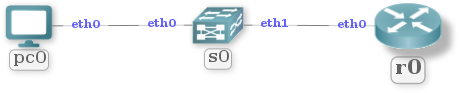
\includegraphics[scale=0.7]{./img/vmc_scene1.png}
  \caption{Use case 1.}
  \label{img:vmc_scene1}
\end{figure}

And here is the VMC associated command

\begin{verbatim}
{
  "workspace" : 12,
  "parameters" : [
    {
      "name" : pc0,
      "type" : pc,
      "network" : [
        {
          "interface" : eth0,
          "collision-domain" : A
        }
      ]
    }, {
      "name" : s0,
      "type" : switch,
      "network" : [
        {
          "interface" : eth0,
          "collision-domain" : A
        }, {
          "interface" : eth1,
          "collision-domain" : B
        }
      ]
    }, {
      "name" : r0,
      "type" : router,
      "network" : [
        {
          "interface" : eth0,
          "collision-domain" : B
        }
      ]
    }
  ]
}
\end{verbatim}

Figure \ref{img:vmc_scene2} is a more elaborated example. Notice that hubs are not represented by a virtual machine but for a single collision domain which is common to all virtual machines connected to it.

\begin{figure}[h!]
  \centering
    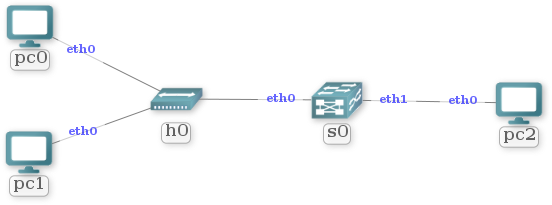
\includegraphics[scale=0.7]{./img/vmc_scene2.png}
  \caption{Use case 2.}
  \label{img:vmc_scene2}
\end{figure}

Next it is the VMC associated command.

\begin{verbatim}
{
  "workspace" : 12,
  "parameters" : [
    {
      "name" : pc0,
      "type" : pc,
      "network" : [
        {
          "interface" : eth0,
          "collision-domain" : A
        }
      ]
    }, {
      "name" : pc1,
      "type" : pc,
      "network" : [
        {
          "interface" : eth0,
          "collision-domain" : A
        }
      ]
    }, {
      "name" : s0,
      "type" : switch,
      "network" : [
        {
          "interface" : eth0,
          "collision-domain" : A
        }, {
          "interface" : eth1,
          "collision-domain" : B
        }
      ]
    }, {
      "name" : pc2,
      "type" : pc,
      "network" : [
        {
          "interface" : eth0,
          "collision-domain" : B
        }
      ]
    }
  ]
}
\end{verbatim}

\subsubsection{VMC Stop}
This command is used to stop one or several virtual machines. Next it is the format of this command.

\begin{verbatim}
{
  "workspace" : Integer,
  "parameters" : [
    {
      "name": String,
    }
    ...
  ]
}
\end{verbatim}

Next command will stop machines the machine \textit{pc1} and \textit{s0} represented by the figure \ref{img:vmc_scene2}

\begin{verbatim}
{
  "workspace" : 12,
  "parameters" : [
    {
       "name": pc1
    }, {
       "name": s0
    }
  ]
}
\end{verbatim}

Notice that we could have used just an array of strings containing the names of the virtual machines to stop, but adding it as an object will make it easy to extend the protocol to be able to include additional parameters inside the object without requiring to make any changes in the parsing logic on the server side.

\subsection{How to create new drivers to manage virtual machines}
This section will explain how you can extend virtual machine manager daemon so as to create your own drivers. These drivers are designed to manage a specific virtualization technology. By default, the daemon comes with a built-in plug-in that manages Netkit, but other ones can be implemented too. In this section you will learn how to get this job done.

Download the source code of the virtual machine manager daemon as it was explained in section \ref{sec:Source} so that we can start hacking in the code.

\begin{verbatim}
$ cd /usr/src/weblab
$ git clone https://github.com/netlab-libresoft/vmmanager.git
\end{verbatim}

Firstly, you have to create a new directory in lib/drivers with the name of your driver. In that directory there must be a package.json file describing your driver. Next it is the netkit package.json configuration file.

\begin{verbatim}
{
  "name": "netkit",
  "description": "Netkit virtual machine driver",
  "version": "0.0.2",
  "author": "Santiago Carot-Nemesio",
  "main": "./netkit.js"
}
\end{verbatim}

In this file, you must declare the name of your driver, a brief description, the current version, who the author is, and which the main file is. Above example indicates that the main file is netkit.js. That file will do the necessary stuff to manage Netkit according to the VMC requests that might be routed to it.

Next there is the directory structure your plug-in must follow:

\begin{figure}[h]
\dirtree{%
.1 netlabmanager.
.2 lib.
.3 drivers.
.4 custom\_driver.
.5 package.json.
.5 main.js.
}
\end{figure}

With all this information, the daemon will try to load at boot time the main file specified in the configuration file that must exist in your driver directory. Next thing you have to do is to provide a Driver object that inherits from Driver class. This class is declared in lib/driver.js and it is exported in file netkit.js using the next statement.

\begin{verbatim}
module.exports = Netkit;
\end{verbatim}

Driver class provide the main functions that will be used to manage your driver, you should implement all of them with the proper stuff to control the underlying virtualiaztion technology you are developing.

See lib/driver.js file for more details.

\subsection{Enhancing the netlab manager daemon functionality}
In this section we are going to explain how you can extend the functionality of this daemon in case you want to provide a new feature in the platform. Remember that netlab manager daemon is in charge of synchronizing all modules connected trough RabbitMQ, furthermore, it is the only one which can connect to the data base, so whenever you want to provide a new feature that involves either synchronizing any module or accessing to the data stored in the data base, you will have to hack in this daemon.

There are many design reason to centralize the access to the data base just in one module, the main one is concerning the source code maintainability. In order to grant the access to the data base it is required to keep the data base schema updated. On the one hand, the data base schema is shared with Netlab Rails application, so any change done in Netlab must be updated and replicated in this daemon to grant the proper access to any piece of data concerning a file or a column in the data base. Having this fact into account, it makes sense that the fewer modules you have to update whenever a change in is done, the better.

So if any of your modules requires a piece of information that it is stored in the data base, you should extend this daemon to provide the proper API to get it using RabbitMQ. Fortunately, Netlabmanager makes it easy by providing a mechanism called \textit{handler}. So you will only need to develop a new handler to have any new feature done. Let's see how it can be done.

Download the source code of the netlab manager daemon just as it was explained in section \ref{sec:Source} so that we can start hacking in the code.

\begin{verbatim}
$ cd /usr/src/weblab
$ git clone https://github.com/netlab-libresoft/netlabmanager.git
\end{verbatim}

A handler is just an instance of an object which inherits from class ServiceHandler. This class is defined in lib/netlabmanager.rb. Here you can see how it looks like.

\begin{verbatim}
class ServiceHandler
  def start
    #TODO: Implement in inherited class
  end

  def stop
    #TODO: Implement in inherited class
  end
  ...
end
\end{verbatim}

Start method will be called in your object once the daemon has started. You will have to set all initialization code here, for example, source code in charge of publishing a new channel in the message system so that other modules can send you messages, etc.

Stop method will be called before the daemon shuts down, here it is the right place to free resources you have set up when the start method was first called.

Handler are stored in lib/handlers directory, so all you need is to copy your handler file there. The netlab manager daemon will instantiate your handler object at boot time.

Next it is the basic structure you handler should have:

\begin{verbatim}
# Next line is just required if you want to use events 
# in order to communicate with other handlers
require 'netlabevent'

# All handlers must be in NetlabHandler module
module NetlabHandler

  # The new handler must inherit from ServiceHandler
  class MyHandler < NetlabManager::ServiceHandler
  
    def start
      # Your initialization stuff goes here
      ...
    end
    
    def stop
      # Release resources taken by your handler
      ...
    end
end
\end{verbatim}

\subsection{Extending the streaming server to provide new sources of data}
This section will explain how to modify the streaming server module to provide new sources of streaming data to your clients.

The streaming server is an Express application built over Node.js, so you should be familiarized with this framework before you can start making changes here. Moreover, Socket.IO library is used to send streaming data to user's web browser, so you should have a read to its APIs to understand some concepts introduced in this section.

Enhancing the streaming server functionality is such an easy task once you understand how Socket.IO works. This library provides the concept of \textit{name space}. Such as its own name indicates, it allows you to multiplex several sources of data in a different space of names. Up until now, only the \textit{workspace} name space is implemented.

Each name space must have its own handler, so that each request which arrived to the server could be managed by a handler which has had to be registered previously.

In order to add a new handler, you must edit the server.js file, the main file of the streaming server. Here you will see that the server implements a chain of initialization callbacks before accepting requests. These callbacks involves some Express application configurations, Socket.IO library initializations, and so on. Once all these callbacks are executed we are ready to register new handlers. In the last callback you can see a comment which invites you to create and register new handlers.

\begin{verbatim}
....
/* Server initialization */
nimble.series([
  function(_callback) {
    /* Configure messaging system */
    ....
  },
  function(_callback) {
    /* Configuration for the application */
    ....
  },
  function(_callback) {
    /* SocketIO server configuration */
    ...
    
    /* General configuration */
    ....
  },
  function(_callback) {
    /* Add name space handlers here */

    /* Attend workspace notifications */
    workspace.attend(io, messenger);

    ...
  }
], function() {
  /* Everything is configured */
  server.listen(9000);
});
\end{verbatim}

Above code summarized the initialization process. All callbacks have been chained using nimble package, it allows you to fire the next callback only when the previous one has finalized. In this way, asynchronous code can be sequentially executed in the time.

As you can see, in order to register a handler all what you need is to provide the socket IO server reference, which will allow you to access to all capabilities provided by this library.

Suppose that we want to create a chat handler to manage messages sent from any user to one another. We could create a new handler file called chat.js inside \textit{lib} subdirectory. This file would export an \textit{attend} function which we would provide the Socket.IO server reference in so as to manage the \textit{chat} name space. We could also provide as many parameters to this function as our chat module might require. Here is the bare bone of our chat handler.

\begin{verbatim}

...
var io;
var chat;
var namespace = '/chat';

exports.attend = function(sockio, ...) {
 io = sockio;
 chat = io
  .of(namespace)
  .on('connection', function (socket) {
    logger.info("Connected new user ");
    ...
  });
}
...
\end{verbatim}

Next thing we have to do is to register the new handler, to do that, all we need is to edit the server.js file in order to register the new handler.

\begin{verbatim}
var chat = require('./lib/chat.js');

/* Server initialization */
nimble.series([
  ...
  function(_callback) {
    /* SocketIO server configuration */
    server = require('http').createServer(app);
    io = require('socket.io').listen(server);
    ...
  },
  ...
  function(_callback) {
    /* Add name space handlers here */

    /* Attend workspace notifications */
    workspace.attend(io, messenger);

    /* Attend chat notifications */
    chat.attend(io, ...);
    ...
  }
], function() {
  /* Everything is configured */
  server.listen(9000);
});
\end{verbatim}

That is it. So far we have prepared the environment for our new \textit{handler}. From now, we can focus in it to develop the required stuff to manage chat conversations among users.

\end{document}